\section{Hosting Laboratory}
In the context of my master's degree, I did 5 months of internship in the SaMova team in IRIT laboratory.\\

The IRIT (\textbf{I}nstitut de \textbf{R}echerche en \textbf{I}nformatique de \textbf{T}oulouse – \textbf{I}nformatics \textbf{R}esearch \textbf{I}nstitute of \textbf{T}oulouse) represents one of the major laboratories of the French research in computer science, with a workforce of more than 700 members including 272 researchers and teachers 204 PhD students, 50 post-doc and researchers under contract and also 32 engineers and administrative employees.\\
The 21 research groups of the laboratory are dispatched in seven scientific themes covering all the computer science domains of today :
\begin{itemize}
 \item 1 : Information Analysis and Synthesis
 \item 2 : Indexing and Information Search
 \item 3 : Interaction, Autonomy, Dialogue and Cooperation
 \item 4 : Reasoning and Decision
 \item 5 : Modelization, Algorithms and High-Performance Calculus
 \item 6 : Architecture, Systems and Networks
 \item 7 : Safety of Software Development
 
\end{itemize}

SAMoVA (\textbf{S}tructuration, \textbf{A}nalysis, \textbf{Mo}delling of \textbf{V}ideo and \textbf{A}udio documents) team, include into the Topic 1 - Information Analysis and Synthesis, focuses its research activities mainly on audiovisual contents. Those works are applied on different kinds of content such as audiovisual content analysis, spoken content analysis, analysis of pathological voice, ...\\

\section{Context}

Since time immemorial, speech has been the most important means of communication among humans. By definition, speech is the ability or act of expressing or describing thoughts, feelings or perceptions through the articulation of words. To do this, humans use their vocal apparatus (lungs, glottis, larynx, tongues, lips, jaws, \dots) to produce "syllables" that fuse to form words and phrases. \newline

Speech recognition allows the captured human voice to be analyzed and transcribed into machine-readable text. Over the past decades, automated speech recognition has become one of the major fields of artificial intelligence and signal processing. Indeed, since the introduction to our daily lives of artificial personal assistants like Siri or Google Assistant, speech recognition systems must answer more complex demands. To achieve this level of complex problem solving, these systems must first understand what the user has said, i.e. do good speech recognition. \newline

Recently, the speech recognition field has benefited from advances in deep learning with neural network methods to improve results and advanced technologies.\\
Speech recognition is traditionally based on two steps (see figure \ref{fig: Speech Procesing expain}):\\
\begin{itemize}
 \item 
First, the raw signal is transformed by a feature extractor to give a new representation of this signal, with more relevant information (generally we use Mel Frequency Cepstral Coefficients as a new representation for speech processing).
\item 
 Second, for speech recognition, this new representation is given as the input of a classifier that will give us the text translation of our input signal.

\end{itemize}
\begin{figure}[h]
 \hspace{-1cm}
 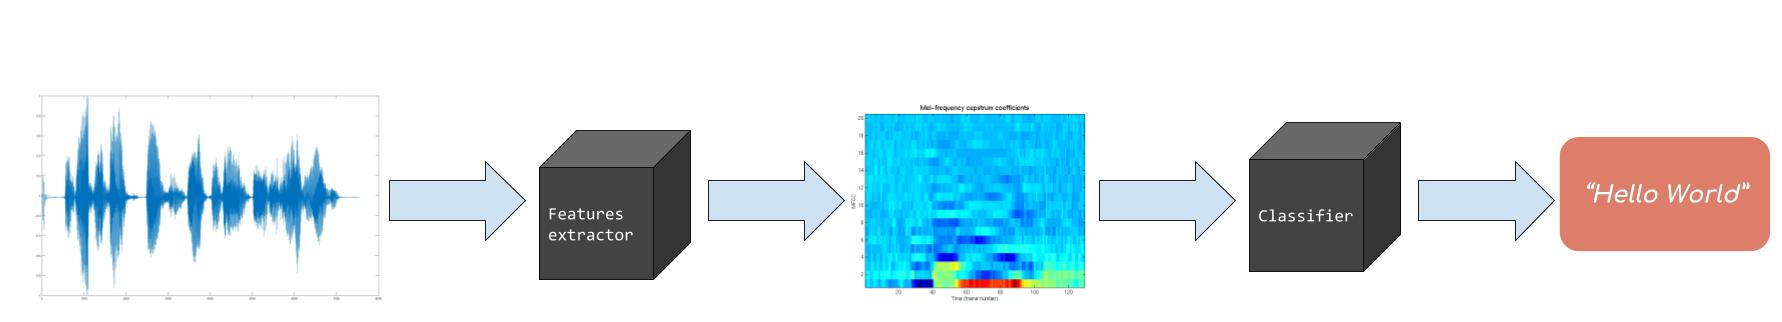
\includegraphics[scale=0.27]{Speech_Processing.jpg}
 % Speech Processing.jpg: 1782x322 px, 72dpi, 62.87x11.36 cm, bb=0 0 1782 322
 \caption{Basic pipeline of speech recognition}
 \label{fig: Speech Procesing expain}
\end{figure}
The goal of my internship is to find a new kind of feature extractor using deep learning and statistical methods. Compare the discriminating power of each of them for signal processing in a generic approach, whether we work on images or sounds. Our work was mainly focused on images using the MNIST dataset since working on the sound level is similar. Indeed the sound signal is transformed into a spectrogram like that will be used as an image to feed the models.

%In order to focus later on only one type of signal: Speech, because work on the spectrograms of the speech signal is the same as work on an image. This is why during this internship we decide to limit our work to the MNIST dataset, a widely used dataset.\\

The chosen methods to replace the traditional feature extractor are:
\begin{itemize}
 \item Auto-Encoder as a Deep learning approach
\item  Sparse Coding a Statistical approach
\end{itemize}
However, the main focus of this internship has been on the statistical methods due to the recent interest of the signal processing community in this kind of method.
\section{Organization}
The present report is organized as follows:
\begin{itemize}
 \item  \textbf{Chapter \ref{chap:SparseCoding}}:  Explain the principle of traditional Sparse Coding, how it is done and give an example on MNIST dataset.
 \item \textbf{Chapter \ref{chap:Discriminative}}: Show the problem with traditional Sparse coding for classification and bring a new solution to obtain a discriminative Sparse code for classification.
 \item \textbf{Chapter \ref{chap:Conv}}: Here, we will explain the natural extension of traditional Sparse Coding to handle shift-variance.
 \item \textbf{Chapter \ref{chap:SupervisedConv}}: As we did in chapter \ref{chap:Discriminative} for traditional Sparse coding, we will explain one method to obtaining discriminatory Sparse coding in Convolution Sparse Coding.
 \item \textbf{Chapter \ref{chap:AE}}: We present the deep learning methods with which we compare Sparse Coding.
 \item \textbf{Chapter \ref{chap:Conclusion}}: Explain our results and the different perspectives we have.
\end{itemize}

